\documentclass[../../Problems]{subfiles}
\begin{document}
\subsection{Staircase Walk}{\label{pp:staircasewalk}}
Consider a grid with $m$ horizontal lines and $n$ vertical lines. A Staircase Walk is defined as the path from bottom-left corner of the grid to the top right corner by walking along the lines; so, the person is constrained to move only in positive $x$ or positive $y$ direction.
\begin{figure}[H]
	\centering
	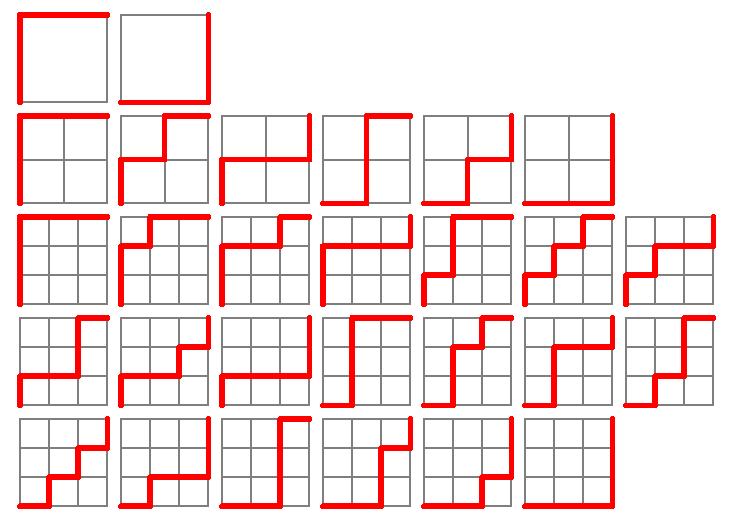
\includegraphics[width = 0.4\linewidth]{Staircase Walk.pdf}
	\caption{Example walks for case $m=n=1\ (\#2),\ m=n=2\ (\#6),\ m=n=3\ (\#20)$ (\href{https://mathworld.wolfram.com/StaircaseWalk.html}{Image Source})}
	\label{fig:staircasewalk}
\end{figure}
\vspace{-1em}
\textbf{Problem Statement:}\\
Find the number of possible \emph{Staircase Walks} for a given $m,n$ (for all test cases).
\begin{testcasesFunction}
	{$t$ \hfill(number of test cases, an integer)\\
	$m_1\ n_1\ \quad m_2\ n_2\ \quad \ldots\quad m_t\ n_t$ \hfill($t$ space seperated integer pairs for each testcase)}
	{Number of Staircase Walks for $m_i, n_i$  \hfill(each test case on a newline)}
	{$1 \leq m_i, n_i \leq 15$}
	{\texttt{int staircase\_walks(int m, int n)} -- returns the number of staircase walks for $m,n$.}
	{6\\1 1\quad 2 5\quad 6 3\quad 7 10\quad 13 8\quad15 15}
	% {11\\1 1\quad 2 2\quad 3 3\quad 5 5\quad 10 10\quad 15 15\quad 2 5\quad 3 3\quad 6 3\quad 7 10\quad 17 8\quad}
	{1\\5\\21\\5005\\50388\\40116600}
	{https://github.com/paramrathour/CS-101/tree/main/Starter Codes/Staircase Walk.cpp}
\end{testcasesFunction}
\begin{funvideo}
\href{https://youtu.be/dQXVn7pFsVI}{The Devil's Staircase -- PBS Infinite Series}
\end{funvideo}
\end{document}